%\documentclass{minimal}
%\usepackage[pdftex,active,tightpage]{preview}
%\usepackage{tikz}
%\begin{document}
%\begin{preview}
%%%%%%%%%%%%%%%%%%%%%%%%%%%%%
	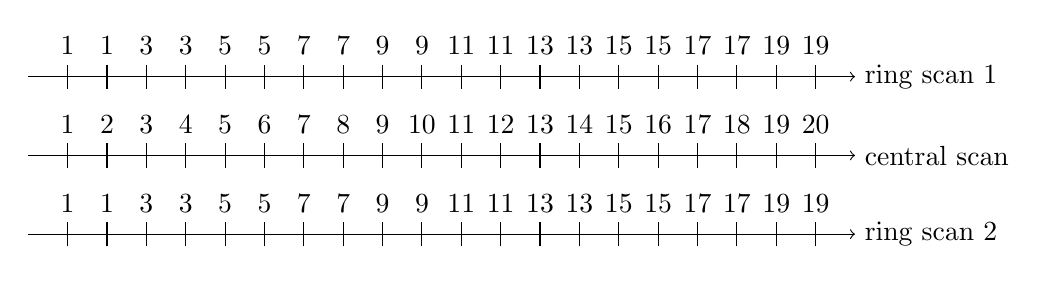
\begin{tikzpicture}[scale=0.5]
	%
	\def\linegap{2}%1.6181229773462783171521035598706}
	\def\length{20}
	\def\ticklength{.309}
	%
	\foreach \y/\label in {0/central scan,\linegap/ring scan 1,-\linegap/ring scan 2}%
		\draw [->] (0,\y) -- (\length+1,\y) node [anchor=west] {\label} ;
	\foreach \x in {1,...,\length}
		\draw (\x,0-\ticklength) -- (\x,0+\ticklength) node [anchor=south] {\x};
	\foreach \z in {1,3,...,\length}
		\draw (\z,\linegap-\ticklength) -- (\z,\linegap+\ticklength) node [anchor=south] {\z}
		(\z+1,\linegap-\ticklength) -- (\z+1,\linegap+\ticklength) node [anchor=south] {\z};
	\foreach \z in {1,3,...,\length}
		\draw (\z,-\linegap-\ticklength) -- (\z,-\linegap+\ticklength) node [anchor=south] {\z}
		(\z+1,-\linegap-\ticklength) -- (\z+1,-\linegap+\ticklength) node [anchor=south] {\z};
	\end{tikzpicture}
%%%%%%%%%%%%%%%%%%%%%%%%%%%%%
%\end{preview}
%\end{document}
